\begingroup
\renewcommand{\baselinestretch}{1}\selectfont
% Local, reusable vector figure styles. Units are centimetres.
\tikzset{
 thesis block/.style={draw=black,line width=.65pt,align=center,inner sep=5pt,font=\sffamily\fontsize{10}{12}\selectfont},
 thesis hw/.style={thesis block,fill=black!9},
 thesis sw/.style={thesis block,fill=white},
 thesis memory/.style={thesis block,double,double distance=1pt,fill=black!3},
 thesis arrow/.style={->,>=stealth,line width=.7pt},
 thesis transfer/.style={<->,>=stealth,line width=.7pt},
 thesis note/.style={align=center,font=\sffamily\fontsize{9}{11}\selectfont,inner sep=3pt},
 thesis title/.style={thesis note,font=\sffamily\bfseries\fontsize{10}{12}\selectfont}
}

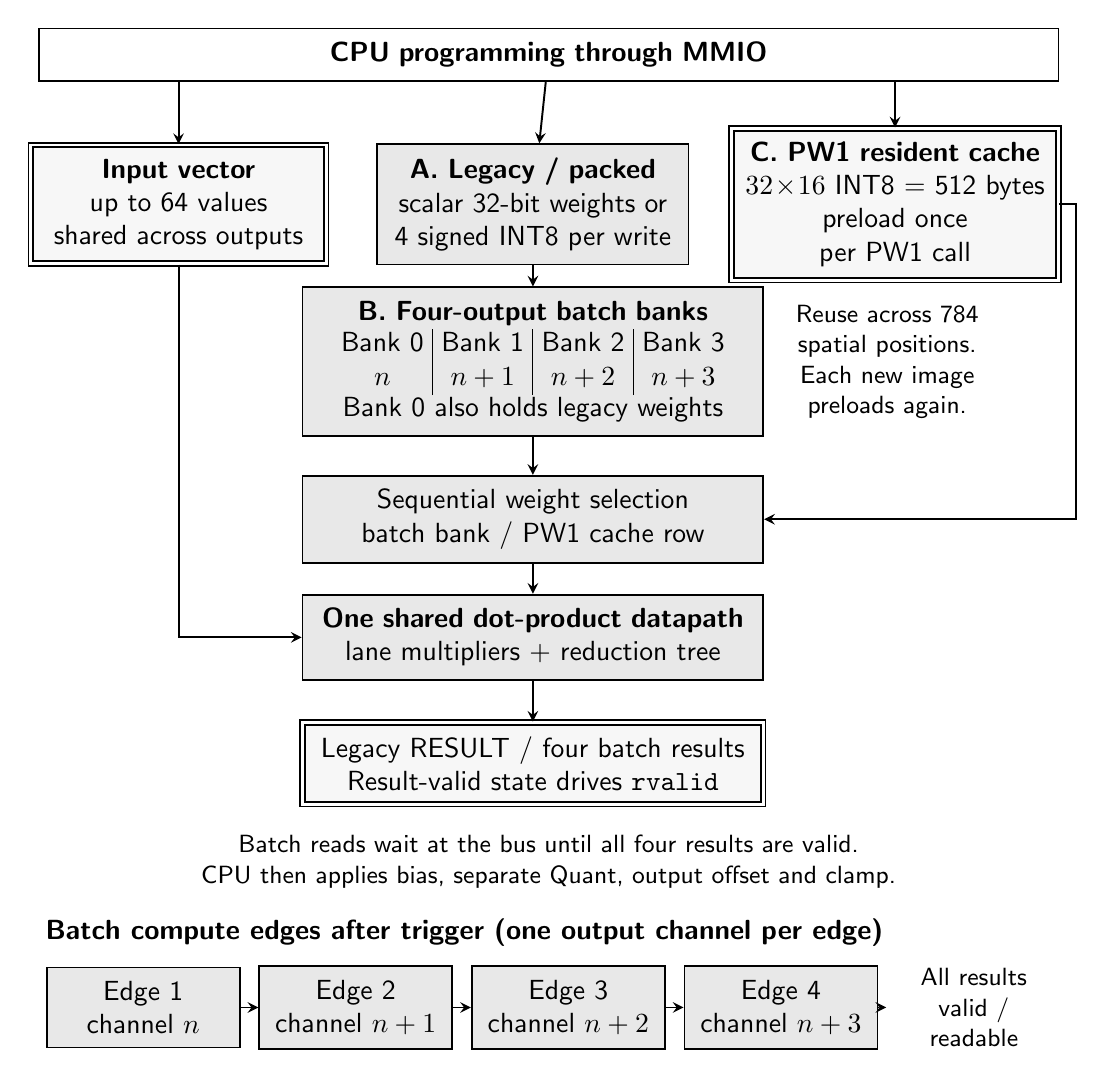
\begin{tikzpicture}[x=1cm,y=1cm]

\node[thesis sw,text width=12.6cm] (cpu) at (6.6,0) {\textbf{CPU programming through MMIO}};
\node[thesis memory,text width=3.4cm,minimum height=1.15cm] (input) at (1.9,-1.9) {\textbf{Input vector}\\up to 64 values\\shared across outputs};
\node[thesis hw,text width=3.6cm,minimum height=1.15cm] (a) at (6.4,-1.9) {\textbf{A. Legacy / packed}\\scalar 32-bit weights or\\4 signed INT8 per write};
\node[thesis memory,text width=3.8cm,minimum height=1.15cm] (cache) at (11,-1.9) {\textbf{C. PW1 resident cache}\\$32\times16$ INT8 = 512 bytes\\preload once per PW1 call};
\draw[thesis arrow] (cpu.south -| input)--(input);
\draw[thesis arrow] (cpu)--(a);
\draw[thesis arrow] (cpu.south -| cache)--(cache);
\node[thesis hw,text width=5.5cm] (banks) at (6.4,-3.9) {\textbf{B. Four-output batch banks}\\\setlength{\tabcolsep}{3pt}\begin{tabular}{c|c|c|c}Bank 0 & Bank 1 & Bank 2 & Bank 3\\$n$ & $n+1$ & $n+2$ & $n+3$\end{tabular}\\Bank 0 also holds legacy weights};
\draw[thesis arrow] (a)--(banks);
\node[thesis hw,text width=5.5cm] (select) at (6.4,-5.9) {Sequential weight selection\\batch bank / PW1 cache row};
\draw[thesis arrow] (banks)--(select);
\draw[thesis arrow] (cache.east)--(13.3,-1.9)--(13.3,-5.9)--(select.east);
\node[thesis note,text width=3.4cm] at (10.9,-3.9) {Reuse across 784 spatial positions.\\Each new image preloads again.};
\node[thesis hw,text width=5.5cm,minimum height=.9cm] (mac) at (6.4,-7.4) {\textbf{One shared dot-product datapath}\\lane multipliers + reduction tree};
\draw[thesis arrow] (select)--(mac);
\draw[thesis arrow] (input.south)--(1.9,-7.4)--(mac.west);
\node[thesis memory,text width=5.5cm] (out) at (6.4,-9) {Legacy RESULT / four batch results\\Result-valid state drives \texttt{rvalid}};
\draw[thesis arrow] (mac)--(out);
\node[thesis note,text width=12.8cm] at (6.6,-10.25) {Batch reads wait at the bus until all four results are valid.\\CPU then applies bias, separate Quant, output offset and clamp.};
\node[thesis title,anchor=west] at (.1,-11.15) {Batch compute edges after trigger (one output channel per edge)};
\foreach \x/\edge/\ch in {1.45/1/n,4.15/2/{n+1},6.85/3/{n+2},9.55/4/{n+3}}{
 \node[thesis hw,text width=2.1cm] (e\edge) at (\x,-12.1) {Edge \edge\\channel $\ch$};
}
\draw[thesis arrow] (e1)--(e2); \draw[thesis arrow] (e2)--(e3); \draw[thesis arrow] (e3)--(e4);
\node[thesis note,text width=2cm] (valid) at (12,-12.1) {All results\\valid / readable};
\draw[thesis arrow] (e4)--(valid);

\end{tikzpicture}
\endgroup
